\usetikzlibrary{calc,arrows.meta}%
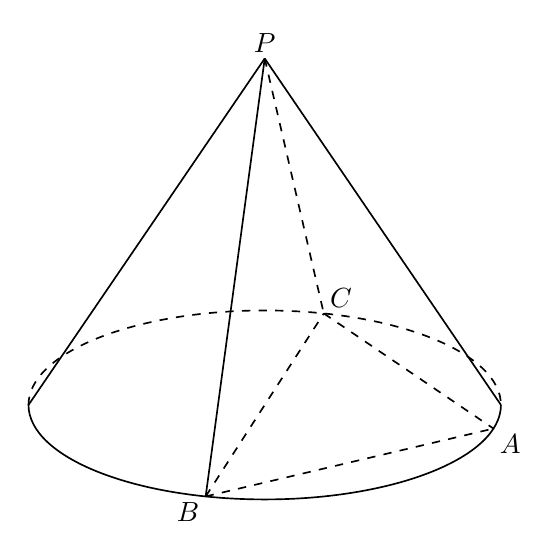
\begin{tikzpicture}[x=1cm,y=1cm,font=\normalsize,line width=.6pt,>=Stealth,
  geometry edge/.style={solid,line width=.6pt,draw=black},
  geometry dashed/.style={dashed,line width=.6pt,draw=black},
  geometry label/.style={font=\normalsize,inner sep=2pt}]
\coordinate (P) at (0,4.4);
\coordinate (B) at (-0.75,-1.161895004);
\coordinate (C) at (0.75,1.161895004);
\coordinate (A) at (2.90473751,-0.3);
\draw[geometry edge] (-3,0) arc (180:360:3 and 1.2);
\draw[geometry dashed] (-3,0) arc (180:0:3 and 1.2);
\draw[geometry edge] (P)--(-3,0);
\draw[geometry edge] (P)--(3,0);
\draw[geometry edge] (P)--(B);
\draw[geometry dashed] (P)--(C);
\draw[geometry dashed] (B)--(C);
\draw[geometry dashed] (C)--(A);
\draw[geometry dashed] (B)--(A);
\node[geometry label,above] at (P) {$P$};
\node[geometry label,below left] at (B) {$B$};
\node[geometry label,above right] at (C) {$C$};
\node[geometry label,below right] at (A) {$A$};
\end{tikzpicture}
